\documentclass[tikz, border=5pt]{standalone}
\usetikzlibrary{arrows.meta}

\begin{document}

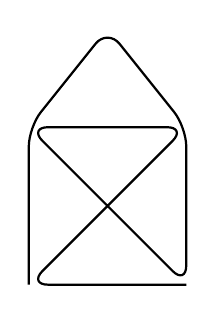
\begin{tikzpicture}
	\draw[thick,rounded corners=7pt]
	(0, 0) -- (0, 2) -- (1, 3.25) -- (2, 2) -- (2, 0) -- (0, 2) -- (2, 2) -- (0, 0) -- (2, 0);
\end{tikzpicture}

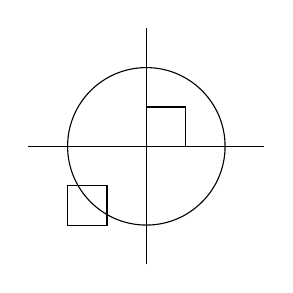
\begin{tikzpicture}
	\draw (-1.5, 0) -- (1.5, 0);
	\draw (0, -1.5) -- (0, 1.5);
	\draw (0, 0) circle [radius=1cm];
	\draw (0, 0) rectangle (0.5, 0.5);
	\draw (-0.5, -0.5) rectangle (-1, -1);
\end{tikzpicture}

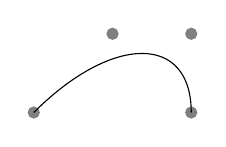
\begin{tikzpicture}
	\filldraw [gray] (0, 0) circle [radius=2pt]
                     (1, 1) circle [radius=2pt]
                     (2, 1) circle [radius=2pt]
                     (2, 0) circle [radius=2pt];
	\draw (0, 0) .. controls (1, 1) and (2, 1) .. (2, 0);
\end{tikzpicture}

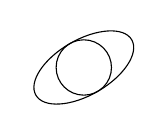
\begin{tikzpicture}
	\draw (0, 0) circle [radius=10pt];
	\draw[rotate=30] (0, 0) ellipse [x radius=20pt, y radius=10pt];
\end{tikzpicture}

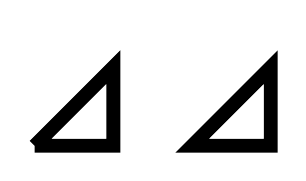
\begin{tikzpicture}[line width=5pt]
	\draw (0, 0) -- (1, 0) -- (1, 1) -- (0, 0);
	\draw (2, 0) -- (3, 0) -- (3, 1) -- cycle;
	\useasboundingbox (0, 1.5);
\end{tikzpicture}


\begin{tikzpicture}
	\shade (0, 0) rectangle (2, 1)
	(3, 0.5) circle (0.5cm);
\end{tikzpicture}

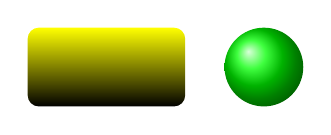
\begin{tikzpicture}[rounded corners,ultra thick]
	\shade[top color=yellow,bottom color=black] (0,0) rectangle +(2,1);
	\shade[ball color=green] (3,.5) circle (.5cm);
\end{tikzpicture}

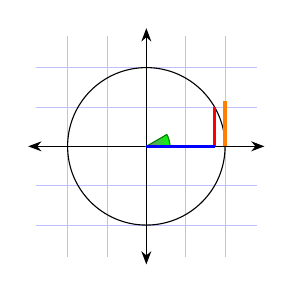
\begin{tikzpicture}[>=Stealth]
	\draw[step=0.5cm, blue!25, very thin] (-1.4, -1.4) grid (1.4, 1.4);
	\draw[<->] (-1.5, 0) -- (1.5, 0);
	\draw[<->] (0, -1.5) -- (0, 1.5);
	\draw (0, 0) circle [radius=1cm];
	\filldraw[left color=gray, right color=green, draw=green!50!black] (0, 0) -- (3mm, 0mm) arc [start angle=0, end angle=30, radius=3mm] -- cycle;
	\draw[red, very thick] (30:1cm) -- +(0, -0.5);
	\draw[blue, very thick] (30:1cm) ++(0, -0.5) -- (0, 0);
	\draw[orange, very thick] (1, 0) -- (1, {tan(30)});
\end{tikzpicture}

\end{document}
